\section{Detection Mechanism}
\label{sec:detection}


In this section, we explain our detection mechanism, starting with an overview of the different steps followed by a detailed description of each step.  
The goal of the detection algorithm is to restore the user's satisfaction in the face of a \drop attack. The key idea of our method is to replace headnodes associated with peer groups of low satisfaction levels. 

Throughput the section, we assume that nodes authenticate their messages using digital signatures. 
% Hatem: trim
% The source keeps track of the verification keys of all participants and can hence establish the authenticity of messages.
The source keeps track of participants' verification keys and can hence establish the authenticity of messages.
In particular, malicious nodes cannot forge responses of honest peers to influence the mechanism. 
We assume that neighboring nodes periodically exchange messages stating that they are neighbors.
These \emph{proofs of neighborhood} are signed and contain a time stamp. 
In this manner, $u$ can proof if $v$ is (or has recently been) its neighbor. 


\begin{table}[ht]
\center
\caption{Acronyms}
\begin{tabular}{|c|l||c|l|}
\hline

\bf{Var.} & \bf{Description}  & \bf{Var.} & \bf{Description} \\\hline\hline
$H_n$ & headnodes in a complaint & $P_n$ & potential candidates list \\\hline
$x$ & no. of malicious peers & $\eta$ & mal. headnodes fraction\\\hline
$BM$ & buffer-map & $MN$ & mal. non-headnodes \\\hline
$\sat$ & peer satisfaction level & $\satThres$ & satisfaction threshold \\\hline
$\minP$ & min. drop responses & $\minDR$ & no. allowed det. \\\hline
\end{tabular}
\label{tab:acronyms}
\vspace{-1mm}
\end{table}



\subsection{Mechanism Overview}
We illustrate the underlying ideas of the detection mechanism in Figure~\ref{detection-blocks}.
When a malicious peer $m$ performs a \drop attack, benign peers $b$ are unable to immediately identify malicious behavior.
Specifically, $m$ never sends the actual $BM$ that represents the chunks it currently possesses, i.e., $m$ is only requesting chunks it already has. 
Thus, detecting a violation in this case is not straight-forward. In particular, nodes are generally unable to identify a suspected attacker based only on local information.
In the remainder of the section, we present a mechanism how nodes can collaboratively identify suspects that are subsequently removed as headnodes.  


The detection consists of four steps, starting with an initial trigger of dissatisfaction at one peer and potentially terminating in replacing one or several headnodes. 
First, when a peer $b$ suspects a \drop attack based on its local observations, $b$ sends a \emph{detection request} to all peers in its neighbor list.
Second, each peer receiving a detection request prepares a reply. 
Third, the initiator $b$ decides based on the received responses if they should file a complaint with the source. 
If $b$ decides to file the complaint, $b$ sends it on behalf of the participating peers in the request. 
Afterwards, the source verifies the complaint, reacts accordingly, and replies to $b$ detailing the steps taken. 
The reaction of the source is either the replacement of one or several headnodes and proposing other potential headnodes or the rejection of the removal request.
Finally, $b$ reacts based on the received reply from the source and then forwards the source's reply to the other participants in the complaint, who in turn execute the same procedure.

The node $b$ bases its decision on whether to initiate a request or forward a complaint on a number of threshold parameters, which we summarize in Table~\ref{tab:acronyms} together with various system parameters governing the attack. 




\begin{figure}
 \centering
 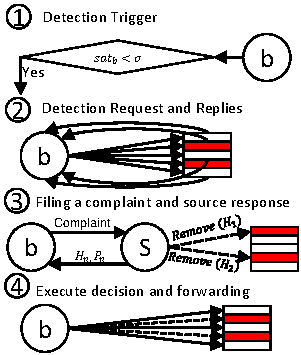
\includegraphics[width=5.5cm,height=5cm]{./Figures/detection.pdf}
 
  \caption{Detection process for \drop. $S$ denotes the source.}
  \vspace{-4.5mm}
\label{detection-blocks} 
\end{figure}


\subsection{Detection Trigger}
\label{Detection-Trigger}


In order to start a detection request, the $b$ has to experience a low level of satisfaction. 
The satisfaction of a peer is defined as the fraction of missed chunks, i.e., the continuity of the stream according to the $Hit/Hit+miss$ chunk ratio.
% \mn[Stef]{how many chunks does the peer consider for that; all during the whole download, only the last $s$ seconds?}
In a nutshell, $b$ starts a detection request if its satisfaction is below a satisfaction threshold $\satThres$.
However, to limit the ability of malicious peers to incorrectly accuse benign peers and increase the load through false detection requests, the concrete conditions that result in a detection request from $b$ are: 

% \begin{itemize}[noitemsep,wide=0pt, leftmargin=\dimexpr\labelwidth + 2\labelsep\relax]

\begin{enumerate}
% \begin{compactenum}
 \item $b$'s current satisfaction level $\sat_b$ is less than the predefined threshold, i.e., $\sat_b < \satThres$.
 \item The number of drop detection requests sent by $b$ in the time interval $t_{det}$ is $< \kappa$. 
%   \mn[Stef]{unclear: is it 'only $\kappa$ requests in last $t_{det}$ timeunits' or 'we divide the time into epochs of length $t_{det}$ and you can only send $\kappa$ per epoch'?}
%   \mn[Hatem]{It is the second one (for every $t_{det}$, only $\kappa$ requests are allowed by peer), I fixed that in the text, please double check.}
 \item $b$ has not initiated or replied to any other \drop detection request that the source has not decided on yet.
% \end{compactenum}
\end{enumerate}
% Hatem: trim
% The latter condition guarantees that peers cannot trigger or participate in multiple detection requests in parallel.
The latter condition guarantees that peers cannot abuse the mechanism via triggering or participating in multiple detection requests in parallel. 
% In addition to limiting the opportunities for abuse, restricting concurrent requests for benign peers is sensible as their low satisfaction level is already noted in their reply to previous requests.
Moreover, restricting concurrent requests for benign peers is sensible as their low satisfaction level is already noted in their reply to previous requests.

\subsection{Processing a Detection Request}
Let $D$ denote the set of queried peers, usually corresponding to the neighbors of the initiator $b$ if $b$ executes the protocol honestly.  
To avoid abuse of the detection mechanism, each node can only participate in $\kappa$ requests for $t_{det}$ timeunits. 
When receiving a detection request, a peer $d \in D$ hence first checks if it can participate in any more requests. 
% \mn[Stef]{Is that correct, or how/when else is that checked?}
% \mn[Hatem]{at the source, if i got your question right}   
    
If so, $d$ replies with its $\sat_d$ and a time stamp, both signed by its private signature key. 
The time stamp prevents the attacker from replaying benign peers' previous (low) satisfaction levels, as only recent satisfaction levels are valid.


\subsection{Filing and Processing a Complaint}

Upon receiving a feedback from its neighbors, $b$ decides whether to file a complaint or not.
If so, the source verifies the complaints and potentially removes some of its headnodes. 

\subsubsection*{Filing a complaint}
$b$ will start processing the replies once all nodes in $D$ have replied or a time-out $t_{replies}$ occurs. 
We assume that the source's address is publicly known and $b$ can send a complaint to the source directly.

$b$ sends a complaint if the average satisfaction level indicated in the responses is below a threshold $\satThres$ and at least $\minP$ peers replied to the request. 
More specifically, let $\sat_1, \ldots ,\sat_z$ are the satisfaction levels expressed in the replies and $\sat_b$ be $b$'s satisfaction level. 
Assuming a sufficient number of replies, $b$ files a complaint to the source if:
\begin{align}
\label{eq:drop_satis_equation}
\frac{1}{z+1}\left( \sat_b + \sum_{i=1}^{z} \sat_i \right) < \satThres. 
\end{align} 
%Hatem: trim
Otherwise, $b$ either starts another detection request depending on $\kappa$ or waits until allowed to send another detection request.
 

Once $b$ decides on filing a complaint according to the aforementioned conditions, $b$ generates a complaint message to the source containing the IDs of all nodes in $D$, recent proofs of neighborhood,  and the received satisfaction levels including signatures and time stamps.  


The reason for requesting at least $\minP$ replies is to prevent a few number of malicious nodes from accusing benign headnodes. By imposing a lower bound on the requested number of replies, a considerable number of malicious nodes has to use one of their $\kappa$ requests. We present an in-depth analysis on how these constraints prevent misuse in Section~\ref{sec:analysis}. 





\subsubsection*{Processing a Complaint at the Source}

The source $s$ first verifies the content of the complaint. First, the source rejects any complaint from a node $b$ that has already participated in $\kappa$ requests. 
If $s$ does not reject the complaint, $s$ then removes any satisfaction levels without valid signatures from the complaint.
Furthermore, $s$ removes any responses from nodes that have exceeded their participation limit or are participating in two complaints at the same time. 

If the remaining valid responses still indicate an average satisfaction level of less than $\satThres$, the source 
\begin{enumerate}
 \item Divides the set of peers in $D$ into two sets $H_n$ and $P_n$, where $H_n$ is assigned as the set of peers participating in the complaint that are already headnodes. 
%  \mn[Stef]{Itemize lists are strange as they are not full sentences but start with a capital letter and end in .}
 \item Removes all peers in $H_n$ from its neighbor set.
 \item Randomly connects to another $|H_n|$ peers. 
 \item Adds peers (excluding peers in $H_n$) from its neighbor list to $P_n$, where $P_n = NeighborList\setminus H_n$ ($NeighborList$ is the set of peers in a neighbor list). 
 \item Sends a \textit{Complaint Reply} to $b$ containing $H_n$ and $P_n$.
\end{enumerate}
 The reason for choosing random new headnodes rather than nodes participating in the complaint is to lower the incentive for complaints by malicious peers. Even if such a complaint is successful, the new headnodes are likely benign, meaning that the malicious nodes did not gain anything from initiating the request apart from increasing the load slightly. 


\subsubsection*{Processing a Complaint Reply \& Forwarding}

Finally, when $b$ receives the \textit{complaint Reply} from the source, $b$ 
\begin{enumerate}
 \item Disconnects from all peers in $H_n$. Note that $b$ does not blacklist peers in $H_n$ from its neighbor list due to the fact that those peers are not proven malicious.
 \item Connects to $|H_n|$ peers from $P_n$, in case $|H_n|>|P_n|$, peers connect to $|P_n|+(|H_n|-|P_n|)$ random peers.
\end{enumerate}
Similarly, $b$ forwards the complaint to the other participants, who in turn execute steps 1 and 2.

\subsection{General Notes}
The detection mechanism does not aim at expelling peers from the system as removing peers as headnodes is highly likely to effectively benefit the system.
Indeed, the only peers that get blacklisted are those who violate the detection mechanism constraints, i.e., participating in more than a single request at a time or initiating more than $\kappa$.
The reason for the lack of harshness of the penalty associated with a detection lies in the potentially high false positive rate for headnodes exhibiting a low performance. 
% These might be accidentally declared to be malicious peers due to not forwarding chunks sufficiently fast. 
% While removing such peers as headnodes is likely to benefit the system, it is not in our interest to ban them from the system. 
In general, the main target of the detection mechanism is to enhance the peers satisfaction level while keeping peer replacements and signaling overhead low.
% \mn[Stef]{Where does it talk about that? who does it when?}


% In Section \ref{sec:eval}, we evaluate these three aspects from various scenarios. 
% Furthermore, we design our protocol such that offers little opportunity for misuse, as we show in the next section. 





